%
% teil1.tex -- Beispiel-File für das Paper
%
% (c) 2020 Prof Dr Andreas Müller, Hochschule Rapperswil
%
% !TEX root = ../../buch.tex
% !TEX encoding = UTF-8
%
\section{Kirchhoffs Gesetz
\label{circuit:section:teil1}}
\rhead{Problemstellung}
Bevor wir die Laplace-Gleichung mithilfe der Lagrange-Funktion herleiten, versuchen wir das auf konventionelle Weise, indem wir  das kirchhoffsche Gesetz benutzen. 
Dafür brauchen wir aber zuerst noch ein paar Erkenntnisse, die hier aufgezeigt werden. Die Stromdichte $\vec{J}$ wird durch
\begin{equation}
	\vec{J}=\frac{\vec{I}}{A}
	\label{circuit:current_density_3}
\end{equation}
definiert. Diese Gleichung besagt, dass die Stromdichte das Verhältnis des Stroms $I$ zur Flächen $A$ ist. 
Das kirchhoffsche Stromgesetz postuliert nun, dass die Summe der in einen Knoten einfliessenden Ströme gleich der Summe der aus diesem Knoten ausfliessenden Ströme in einer Schaltung ist. Dies impliziert, dass es in einem Gleichstromkreis im stationären Zustand keine Ladungsakkumulation an irgendeinem Punkt geben kann. Wir betrachten nun einen dreidimensionalen Schaltkreis, in dem die Leitfähigkeit $\sigma$ im gesamten Bereich von Interesse konstant ist. Die Verallgemeinerung des kirchhoffschen Stromgesetzes im dreidimensionalen Fall besagt, dass die Divergenz der Stromdichte $\vec{J}$ gleich Null ist, es kann kein Strom aus dem Nichts erzeugt werden. Daher gilt 
%\eqref{circuit:current_density_1}.
\begin{equation}
	\nabla \cdot  \vec{J}=0.
	\label{circuit:current_density_1}
\end{equation}

Zudem lässt sich der zusammenhing zwischen dem elektrischen Feld $\vec{E}$ an einem gegebenen Punkt im Raum als negativer Gradient der Potentialfunktion $\phi$ 
\begin{equation}
	\vec{E}=-\nabla \phi
	\label{circuit:current_density_4}
\end{equation}
ausdrücken.

Wenn das elektrische Feld durch $\vec{E}$ repräsentiert wird und wir ein ohmsches Material vorliegen haben, kann die Stromdichte auch als Produkt  
\begin{equation}
\vec{J}=\sigma \vec{E}
\label{circuit:current_density_2}
\end{equation}
beschrieben werden.
Mit dem elektrischen Feld als Gradient von $\phi$ erhalten wir aus der Quellenfreiheit des Stromes \eqref{circuit:current_density_1} und dem ohmschen Gesetz \eqref{circuit:current_density_2} die Differentialgleichung 
\begin{equation}
	\nabla \cdot (\sigma \nabla \phi)=0
	\label{circuit:current_density_5}
\end{equation}
für das Potential $\phi$. Dies kann auch als
\begin{equation}
\nabla^2 \phi=0
\label{circuit:current_density_6}
\end{equation}
geschrieben werden.

\section{Variationsprinizip}
Im nächsten Schritt versuchen wir, die Gleichung \eqref{circuit:current_density_6} mithilfe eines Minimalprinzips herzuleiten. Das Minimalprinzip besagt, dass ein physikalisches System so arbeitet, dass eine bestimmte Größe minimiert wird. In unserem Fall ist diese Größe die Leistung der Schaltung.
Um das Prinzip zu veranschaulichen, betrachten wir eine Parallelschaltung von zwei Widerständen, einem \SI{1}{\kilo\ohm} und einem \SI{2}{\kilo\ohm} Widerstand, wie in Abbildung \ref{fig:circuit_stromzweig} dargestellt. Zudem nehmen wir an, dass der Strom $I_0$ \SI{1}{\ampere} beträgt. 
\begin{figure}
	\centering
	\begin{circuitikz}
		\draw (0,3) to[V, v=$U_0$, i=$I_0$] (0,0);
		\draw (0,3) to[short,-*] (3,3)
		to[R, l=$R_1$, i=$I_1$] (3,0) -- (0,0);
		\draw (3,3) -- (6,3)
		to[R, l=$R_2$, i=$I_2$] (6,0) to[short,-*] (3,0);
	\end{circuitikz}
	\caption{Parallelschaltung von $R_1= \SI{2}{\kilo\ohm}$ und $R_2= \SI{1}{\kilo\ohm}$}
	\label{fig:circuit_stromzweig}
\end{figure}
Der Strom nimmt dabei wie ihnen bekannt ist nicht den Weg des geringsten Wiederstandes sondern den Weg indem die Leistung der Schaltung minimiert wird. D.h. es fliesst nicht der ganze Strom durch den \SI{1}{\kilo\ohm} Widerstand was mit einer Leistung von \SI{1}{\kilo\watt} resultieren würde. Sondern es fliessen zwei Drittel des Stromes durch den \SI{1}{\kilo\ohm} Widerstand und ein Drittel des Stroms durch den zwei Kilo Ohm Widerstand. Was in einer Leistung von $P=  I_1^2 \cdot R_1+  I_2^2 \cdot R_2 =(\SI{0.333}{\ampere})^2\cdot \SI{2}{\kilo\ohm}+(\SI{0.667}{\ampere})^2\cdot \SI{1}{\kilo\ohm} = \SI{666.67}{\watt}$ resultiert und die minimal mögliche Leistung ist, wie es auch in Abbildung \ref{fig:circuit_power} gesehen werden kann oder Mathematisch aufgezeigt werden kann:
Der Strom $I_2$ kann auch als $I_0-I_1$ geschrieben werden, daraus folgt 
\begin{equation}
	P(I_1)=  I_1^2 \cdot R_1+  (I_0-I_1)^2 \cdot R_2.
	\label{circuit:current_circuit_power}
\end{equation}
Um das Minimum zu finden leiten wir nun nach $I_1$ ab und bekommen
\begin{equation}
	\frac{dP}{dI_1} = 2\cdot I_1\cdot R_1 - 2\cdot (I_0 - I_1) \cdot R_2.
	\label{circuit:current_circuit_power1}
\end{equation}
Des weiteren zeigt die zweite Ableitung 
\begin{equation}
	\frac{d^2P}{dI_1^2} = 2\cdot R_1 + 2\cdot R_2
	\label{circuit:current_circuit_power2}
\end{equation}
eindeutig das es sich um ein Minimum handelt da $R_1$ und $R_2$ positiv sind und daher die zweite Ableitung positiv ist. Wenn wir nun die erste Ableitung \eqref{circuit:current_circuit_power1} gleich 0 setzen und auf $I_1$ auflösen bekommen wir
\begin{equation}
	I_1 = \frac{I_0 \cdot R_2}{R_1 + R_2} = \frac{\SI{1}{\ampere} \cdot \SI{1}{\kilo\ohm}}{\SI{2}{\kilo\ohm}+ \SI{1}{\kilo\ohm}}=\SI{0.333}{\ampere}
	\label{circuit:current_circuit_power3}
\end{equation}
und analog
\begin{equation}
	I_2 = I_0-I_1=\SI{1}{\ampere}-\SI{0.333}{\ampere}=\SI{0.667}{\ampere}.
	\label{circuit:current_circuit_power4}
\end{equation}
Somit wurde erfolgreich demonstriert, dass die Verteilung des Stroms in der Schaltung direkt mit der Minimierung der gesamten Leistung korrespondiert.
\begin{figure}
	\centering
	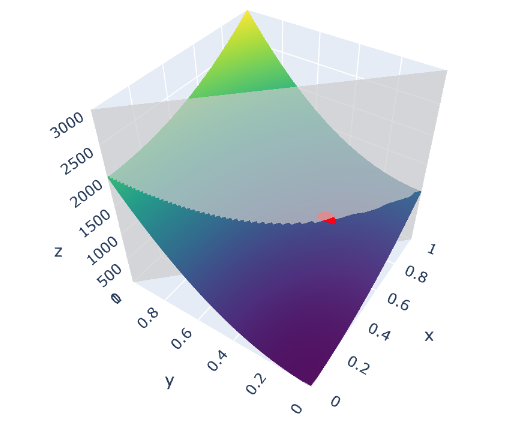
\includegraphics[width=0.7\textwidth]{papers/circuit/two_parrallel_resistors.png}
	\caption{Leistung ($z$-Achse) von zwei parallel geschalteten Widerständen 1 Kilo Ohm ($x$-Achse) und 2 Kilo Ohm ($y$-Achse), in grau dargestellt die Schnittfläche des Stromes von einem Ampere.}
	\label{fig:circuit_power}
\end{figure}
Analog zu dem oben aufgeführten Beispiel können wir die Leistung $P$ in einem von einer Oberfläche $S$ umgebenen Volumen $V$ durch 
\begin{equation}
	P=\int_V \sigma(\nabla \phi)^2 d V
	\label{circuit:current_density_7}
\end{equation}
ausdrücken. Wenn wir nun die Euler-Ostrogradski-Differentialgleichung für \eqref{circuit:current_density_7} bestimmen und lösen gibt uns dies anschliessend die Lösung für die minimale Leistung in einem zweidimensionalen oder dreidimensionalen Raum. D.h. um das Minimum zu finden muss das Integral von \eqref{circuit:current_density_7} minimiert werden. Auf den ersten Blick mag \eqref{circuit:current_density_7} nicht sehr intuitiv erscheinen. Daher könnten wir die Gleichung auch anders formulieren, wie in 
\begin{equation}
	P=\frac{U^2}{R}
	\label{circuit:current_density_8}
\end{equation}
gezeigt, wobei $U^2=\left( \nabla \phi \right)^2$ und $R=\frac{1}{\sigma}$.


\section{Herleitung der Laplace Gleichung}
In diesem Kapitel leiten wir die Laplace-Gleichung her. Die Herleitung basiert auf der Euler-Ostrogradski-Differentialgleichung, die in Gleichung \eqref{buch:felder:ostrogradski:eqn:euler-ostrogradski} dargestellt ist.

Wir beginnen mit Gleichung \eqref{circuit:current_density_7} und wenden darauf die genannte Differentialgleichung an:
\begin{enumerate}
	\item Schritt: Lagrange-Funktion des Problems ohne $\sigma$ (da wir das Minimum suchen und $\sigma$ eine Konstante ist hat $\sigma$ keinen Einfluss auf die Lösung und kann daher weggelassen werden)
	\begin{equation}
		L(U, U_x)= U_x^2 = (U_{x_1}^2+U_{x_2}^2).
	\end{equation}
	\item Schritt: partielle Ableitungen
	\begin{equation}
		\begin{aligned}
			\frac{\partial L}{\partial U}&=0\\
			\frac{\partial L}{\partial U_{x_1}}&=2U_{x_1}\\
			\frac{\partial L}{\partial U_{x_2}}&=2U_{x_2}.\\
		\end{aligned}
	\end{equation}
	\item Schritt: Ableiten nach $x_1$ und $x_2$
	\begin{equation}
		\begin{aligned}
			\frac{\partial}{\partial x_1}\frac{\partial L}{\partial U_{x_1}}(x,\phi,\nabla \phi)=2\frac{\partial \phi}{\partial {x_1}}\cdot \frac{\partial}{\partial x_1},\\
			\frac{\partial}{\partial x_2}\frac{\partial L}{\partial U_{x_2}}(x,\phi,\nabla \phi)=2\frac{\partial \phi}{\partial {x_2}} \cdot \frac{\partial}{\partial x_1}.\\
		\end{aligned}
	\end{equation}
	\item Schritt: Euler-Ostrogradski Differentialgleichung
	\begin{equation}
		0=-\frac{\partial}{\partial x_1}\cdot 2\frac{\partial \phi}{\partial {x_1}}-\frac{\partial}{\partial x_2}\cdot 2\frac{\partial \phi}{\partial {x_2}}=-2\Delta\phi.
	\end{equation}
\end{enumerate}
\subsubsection{Resultat der Anwendung der Theorie der Euler-Ostrogradski-Differentialgleichung}
	\begin{equation}
	\sigma \cdot 2\Delta\phi=0.
	\end{equation}
Wir können nun noch durch $2\sigma$ teilen und bekommen die Laplace-Gleichung aus \eqref{circuit:current_density_6}. Somit wurde gezeigt dass die Laplace-Gleichung auch dem Variationsprinzip gefunden werden kann sowie auch mit den kirchhoffschen Regeln.
%	\begin{equation}
%	\Delta\phi=0=\frac{\partial^2\phi}{\partial x^2}+\frac{\partial^2\phi}{\partial y^2}
%	\label{circuit:laplace1}
%	\end{equation}
	%\begin{equation}
	%	\Delta \phi(x,y)=\frac{\delta^2\phi}{\delta x^2}+\frac{\delta^2\phi}{\delta y^2}=0
	%\end{equation}


\section{Praktische Anwendungen}
In diesem Abschnitt schauen wir uns an, wie die elliptische partielle Differentialgleichung \eqref{circuit:laplace1} numerisch gelöst werden kann und was sie eigentlich genau bedeutet. 

Gleichung \eqref{circuit:laplace1} kann durch die Differenz zweiter Ordnung diskretisiert werden wie in 
\begin{equation}
	f^{\prime \prime}(x) \approx \frac{\delta_h^2[f](x)}{h^2}=\frac{\frac{f(x+h)-f(x)}{h}-\frac{f(x)-f(x-h)}{h}}{h}=\frac{f(x+h)-2 f(x)+f(x-h)}{h^2}.
	\label{circuit:second-order-central}
\end{equation}
\cite{enwiki:1220817436}
Wenn wir das auf unseren zweidimensionalen Fall anwenden benötigen wir Gitterpunkte, welche mit $x_i$ und $y_i$ dargestellt werden können, sowie die Differenz zwischen den beiden Gitterpunkten, was mit $\Delta x$ und $\Delta y$ geschrieben werden kann
\begin{equation}
	\frac{\phi(x_{i+1}, y_j) - 2\phi(x_i, y_j) + \phi(x_{i-1}, y_j)}{(\Delta x)^2} + \frac{\phi(x_i, y_{j+1}) - 2\phi(x_i, y_j) + \phi(x_i, y_{j-1})}{(\Delta y)^2} = 0.
	\label{circuit:discret_equation}
\end{equation}

Nun können wir nach $\phi(x_i, y_j)$ auflösen und bekommen 
\begin{equation}
	\phi(x_i, y_j) = \frac{1}{4}(\phi(x_{i+1}, y_{j}) + \phi(x_{i-1}, y_{j}) + \phi(x_{i}, y_{j+1}) + \phi(x_{i}, y_{j-1})).
	\label{circuit:discret_equation2}
\end{equation}
mit welcher man numerisch die Werte des Potentials in den Gitterpunkten berechnen kann.
%Darum ist die Idee nun nacheinander \eqref{circuit:discret_equation3} auszureichen bis $\phi$ konvertiert.
%\begin{equation}
%	\phi(x_i, y_j) \to \frac{1}{4}(\phi(x_{i+1}, y_{j}) + \phi(x_{i-1}, y_{j}) + \phi(x_{i}, y_{j+1}) + \phi(x_{i}, y_{j-1}))
%	\label{circuit:discret_equation3}
%\end{equation}
\subsubsection{Numerisches Beispiel}
In diesem Beispiel betrachten wir eine leitende Platte mit einer Leitfähigkeit von \SI{0.001}{\siemens\per\meter} und einer Grösse von einem Quadratmeter. Ein spezifischer Bereich der Platte (Quadrat), definiert durch $0.5 < x < 0.7$ und $0.5 < y < 0.7$, wird mit einem Potential von einem Volt belegt, während der Rand der Platte ein Potential von 0 Volt aufweist.
\begin{figure}
	\centering
	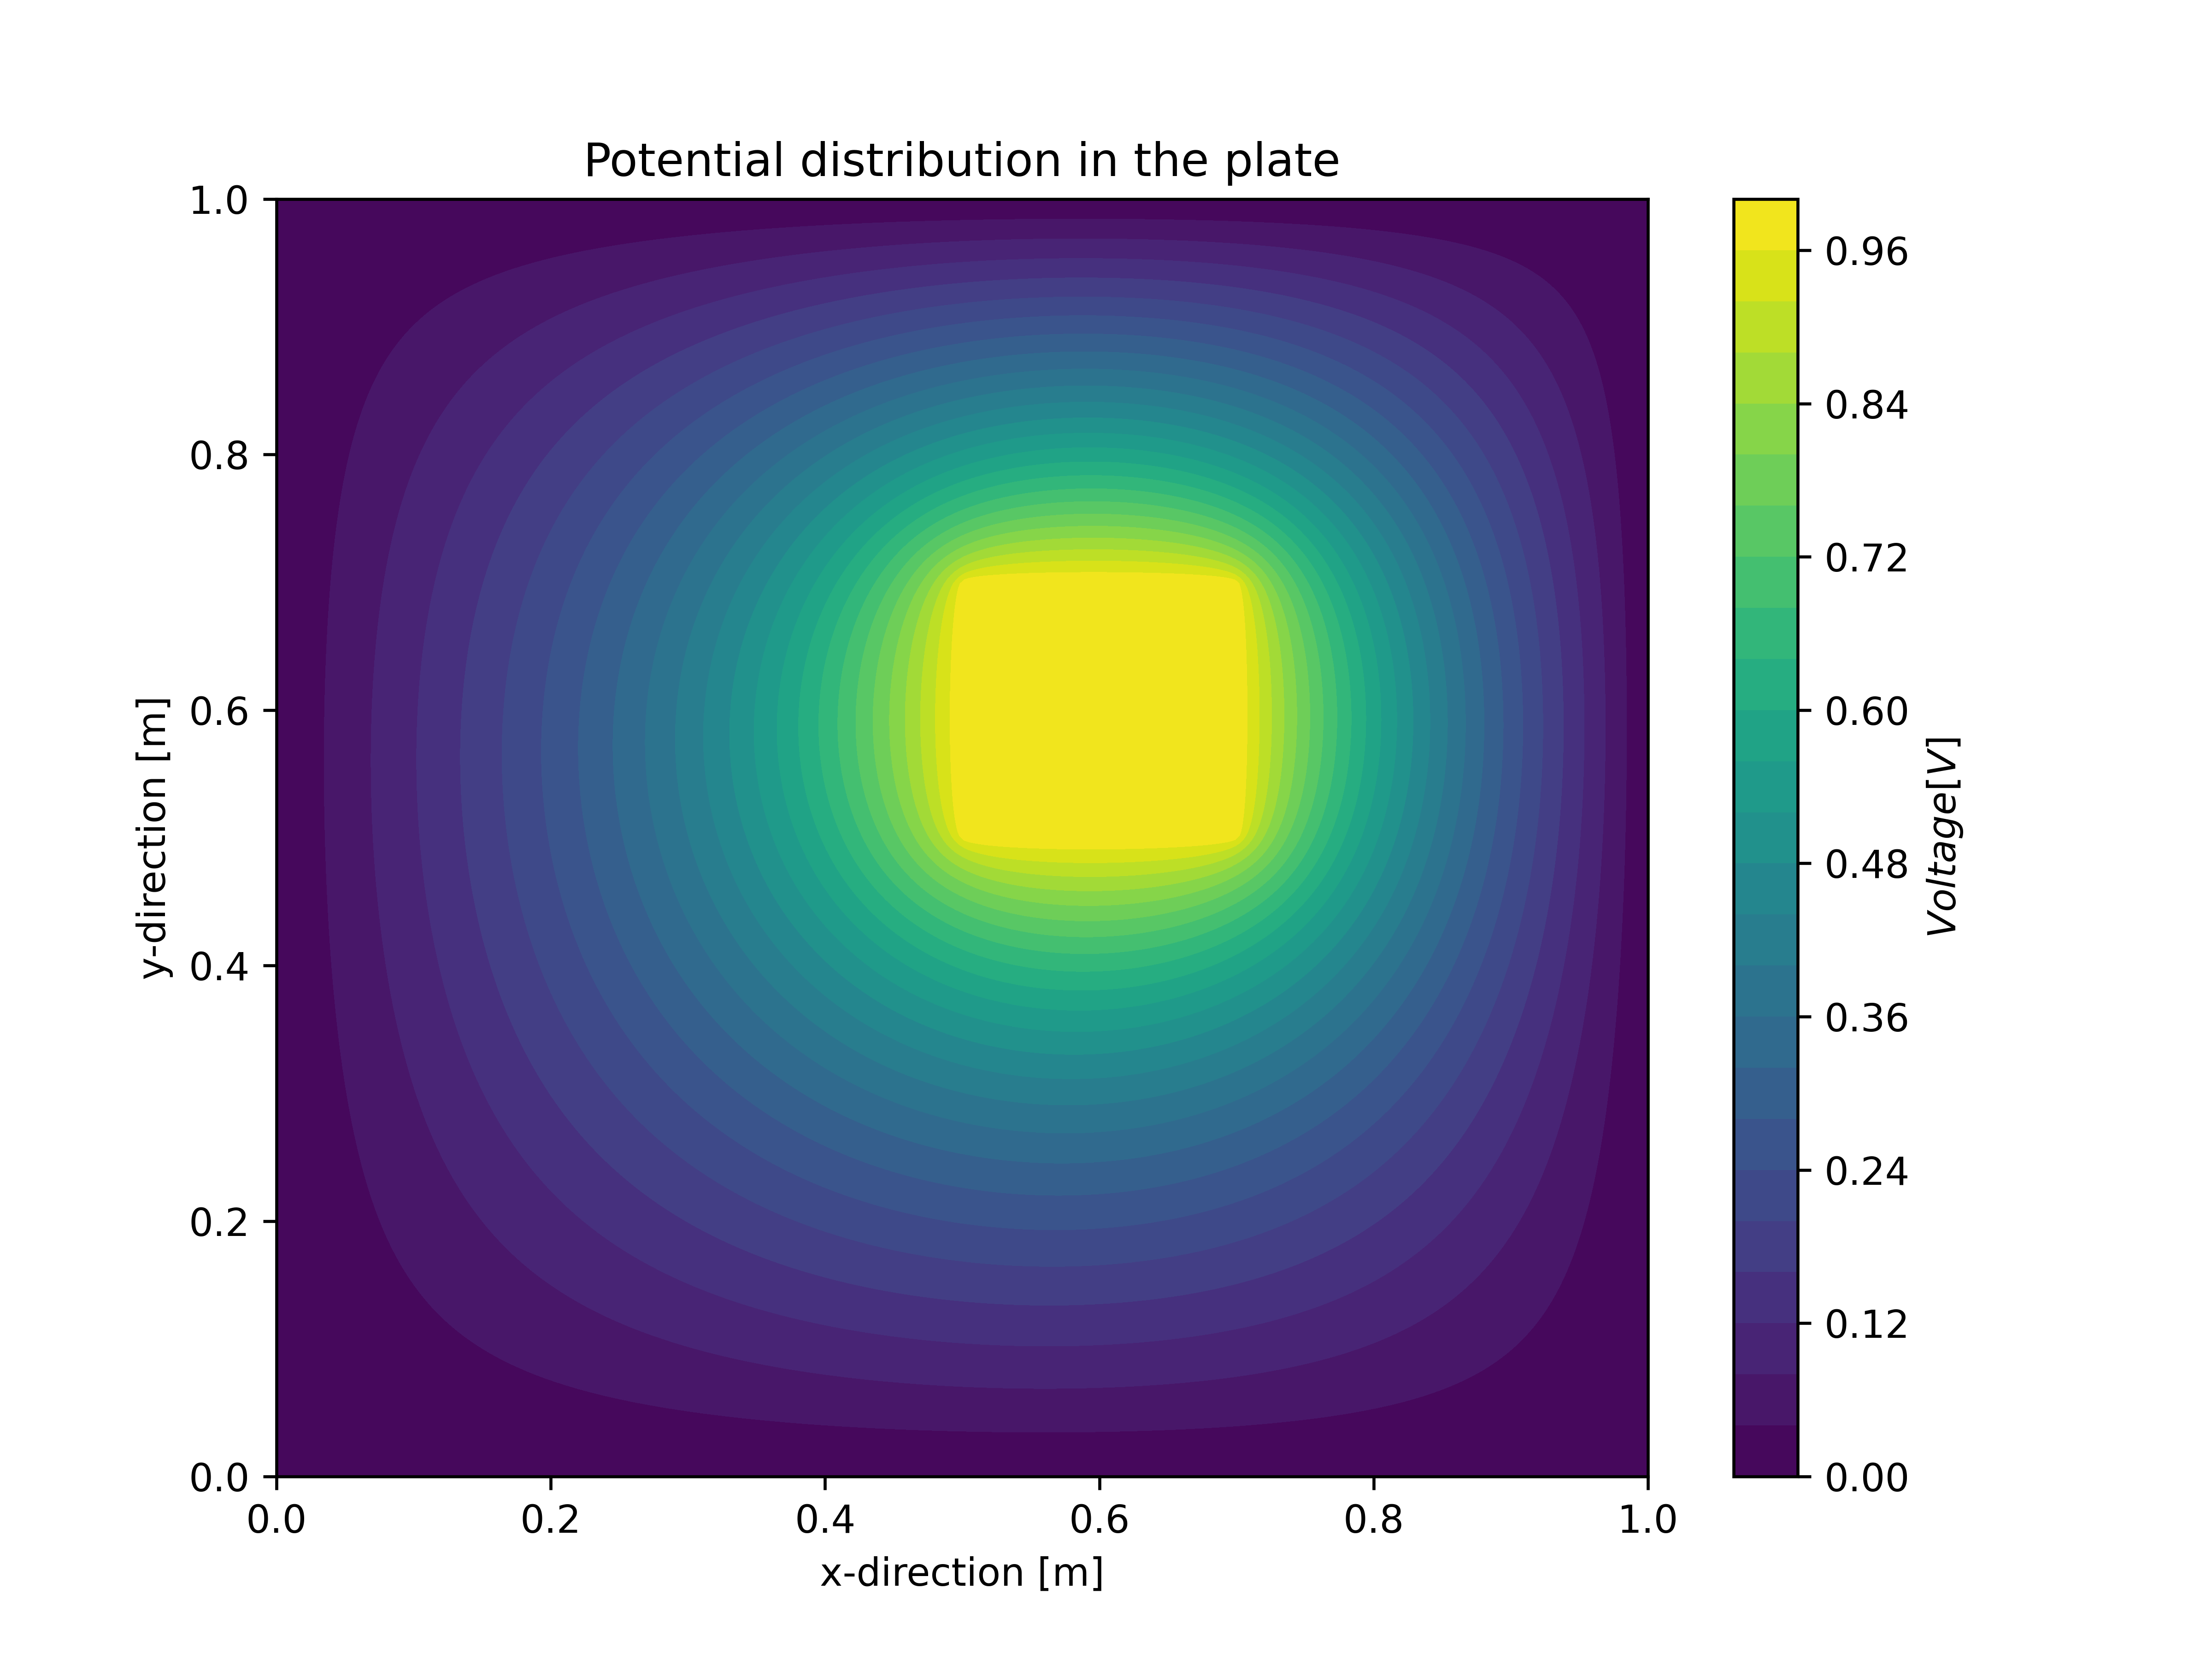
\includegraphics[width=0.99\textwidth]{papers/circuit/potential_distribution.png}
	\caption{Potential-Verteilung auf rechteckiger Platte mit rechteckigem Potential im oberen rechten Bereich und 0 Potential am Rand der Platte \cite{github:AndreasFMueller}}
	\label{fig:potential_distribution}
\end{figure}
Unter Verwendung von Gleichung \eqref{circuit:discret_equation2} zur Berechnung des Potentials, sowie den gegebenen Randbedingungen erhalten wir die in Abbildung \ref{fig:potential_distribution} dargestellte Potentialverteilung. Dies ermöglicht uns, das gesamte Potential auf der Platte zu bestimmen.

Sobald das Potential bekannt ist, können wir mithilfe des Gradienten und Gleichung \eqref{circuit:current_density_7} die Leistungsdichte an jedem einzelnen Punkt berechnen. Dies führt zu den in Abbildung \ref{fig:power_2d} und \ref{fig:power_3d_rectangle} dargestellten Leistungsdichteverteilung.
%die auch im Beispielskript unter folgendem Link \footnote{https://github.com/AndreasFMueller/SeminarVariation/blob/master/buch/papers/circuit/Pr\%C3\%A4sentation.ipynb} gefunden werden können.
\begin{figure}[h]
	\centering
	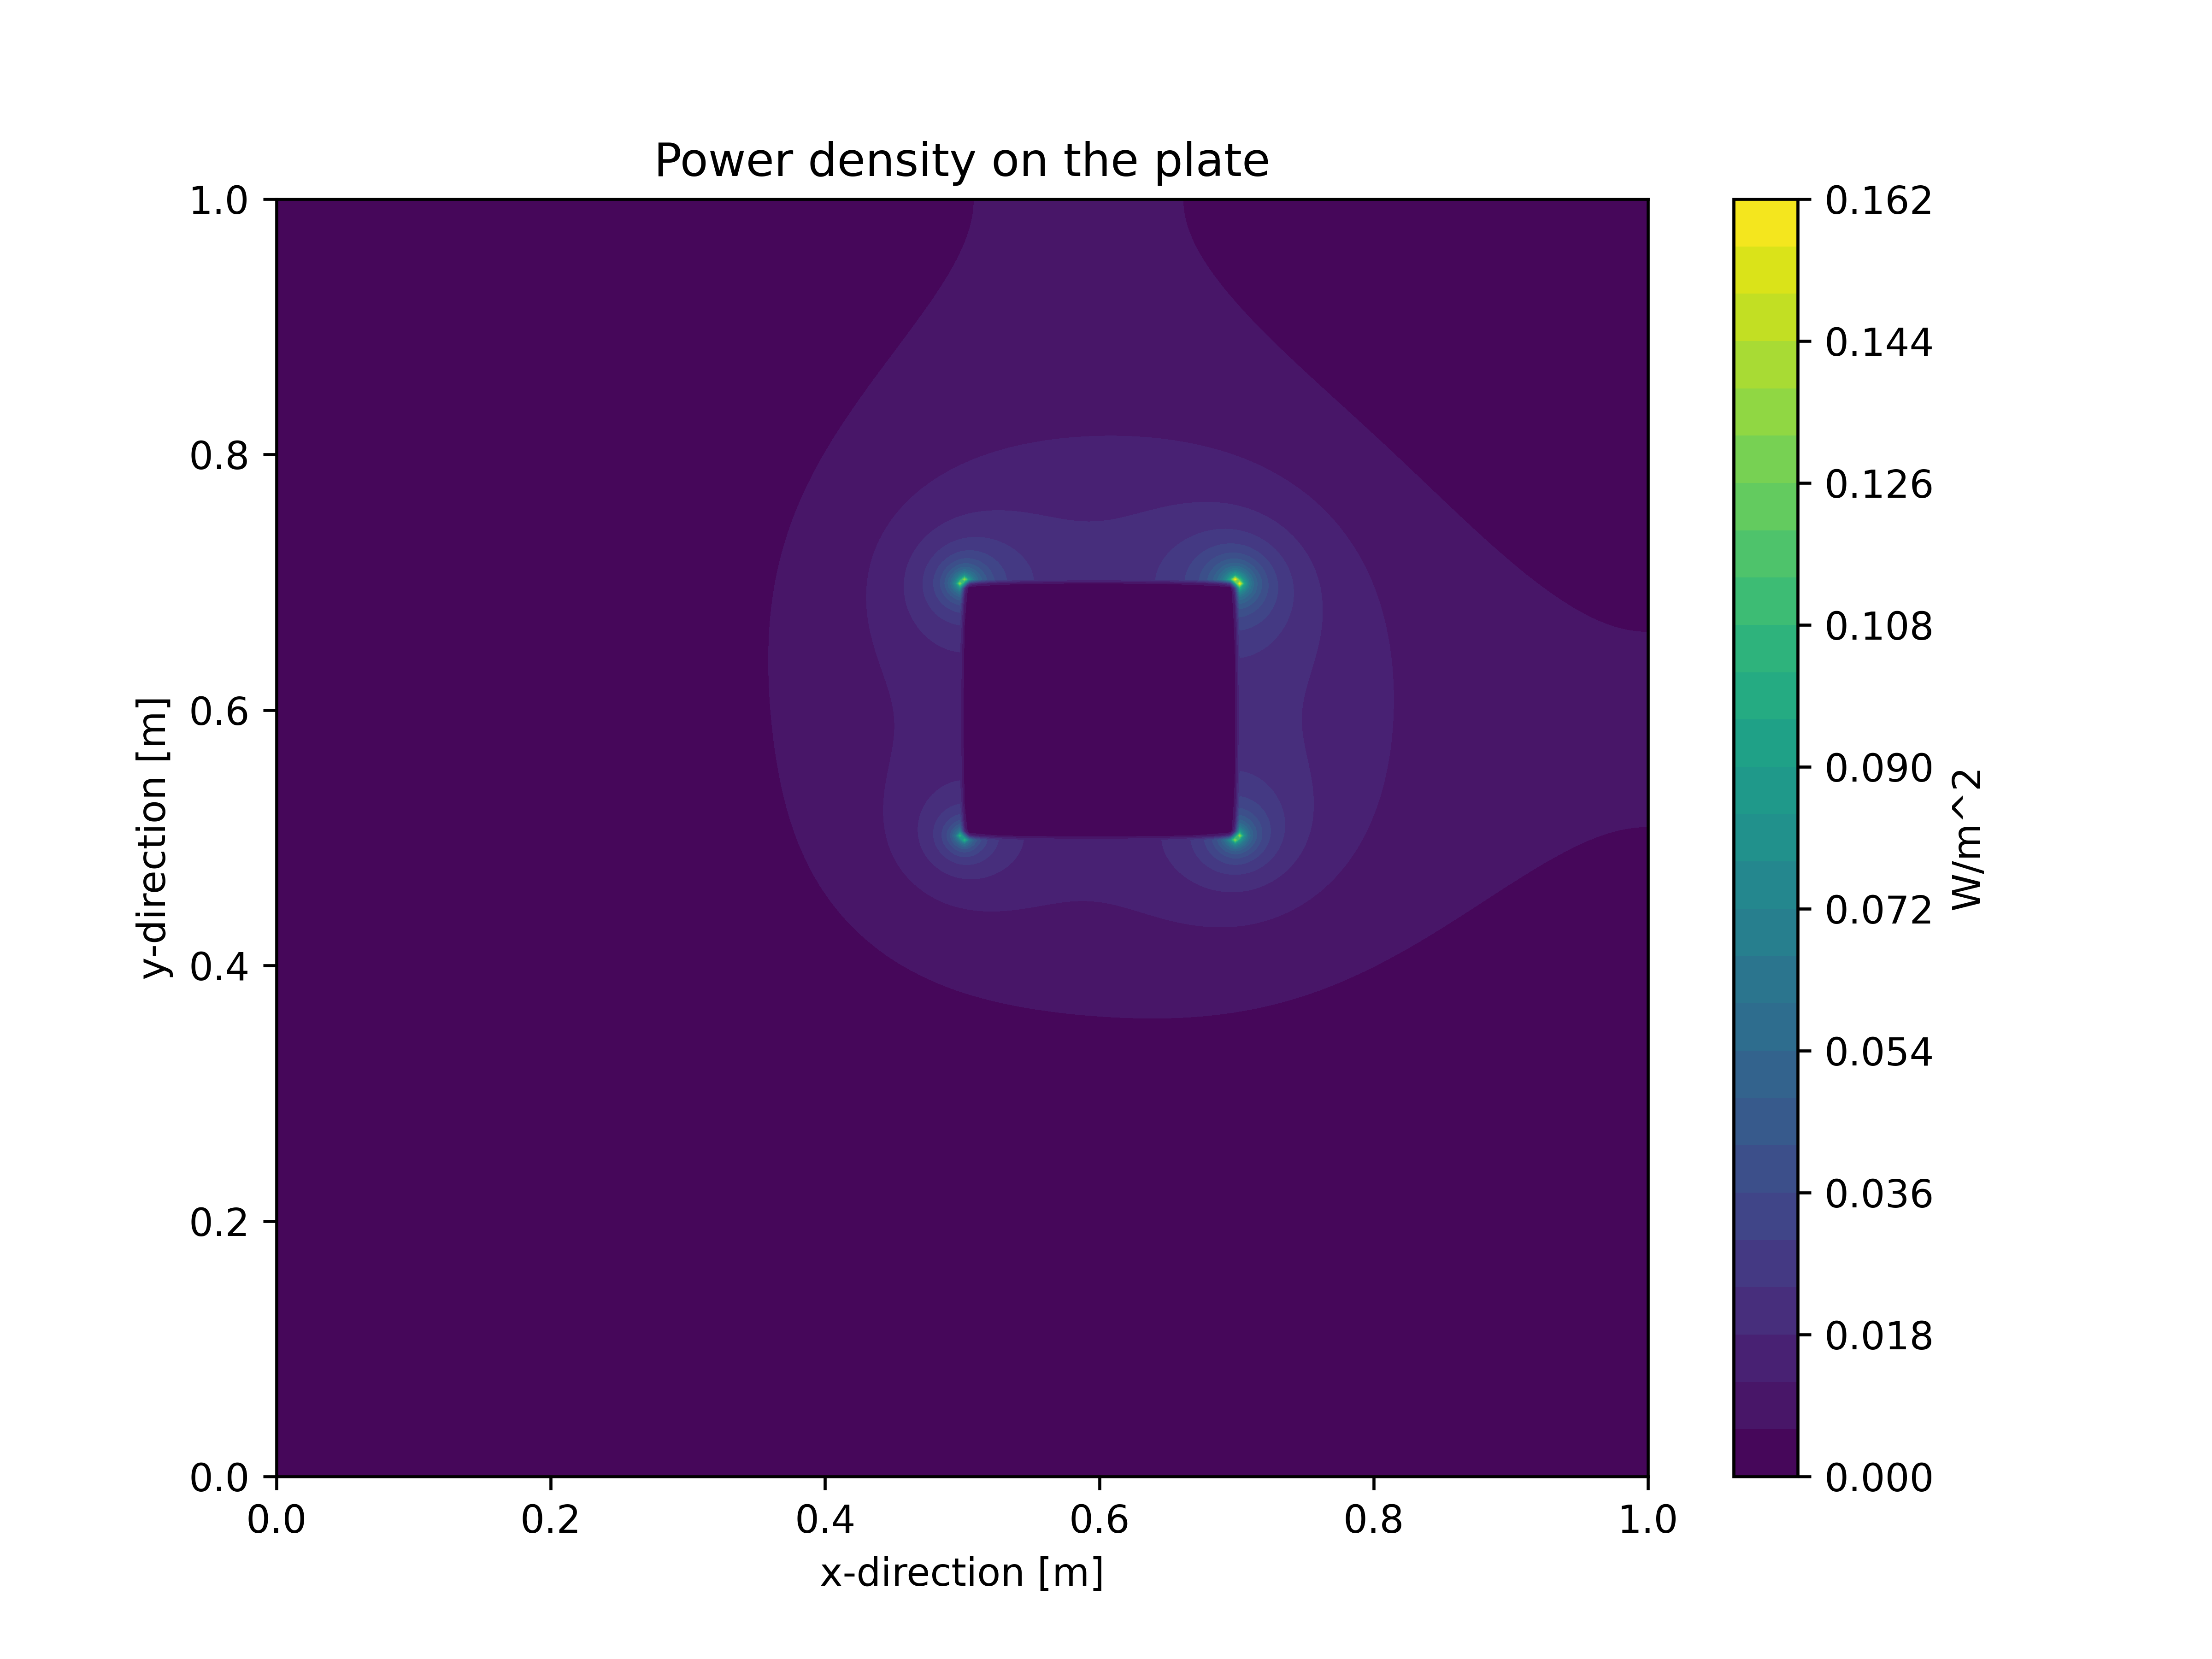
\includegraphics[width=0.99\textwidth]{papers/circuit/power_distribution.png}
	\caption{Leistungsdichte auf rechteckiger Platte mit rechteckigem Potential im oberen rechten Bereich und 0 Potential am Rand der Platte. (Code für die Generierung des Plots kann in \cite{github:AndreasFMueller} gefunden werden.)}
	\label{fig:power_2d}
\end{figure}
\begin{figure}[h]
	\centering
	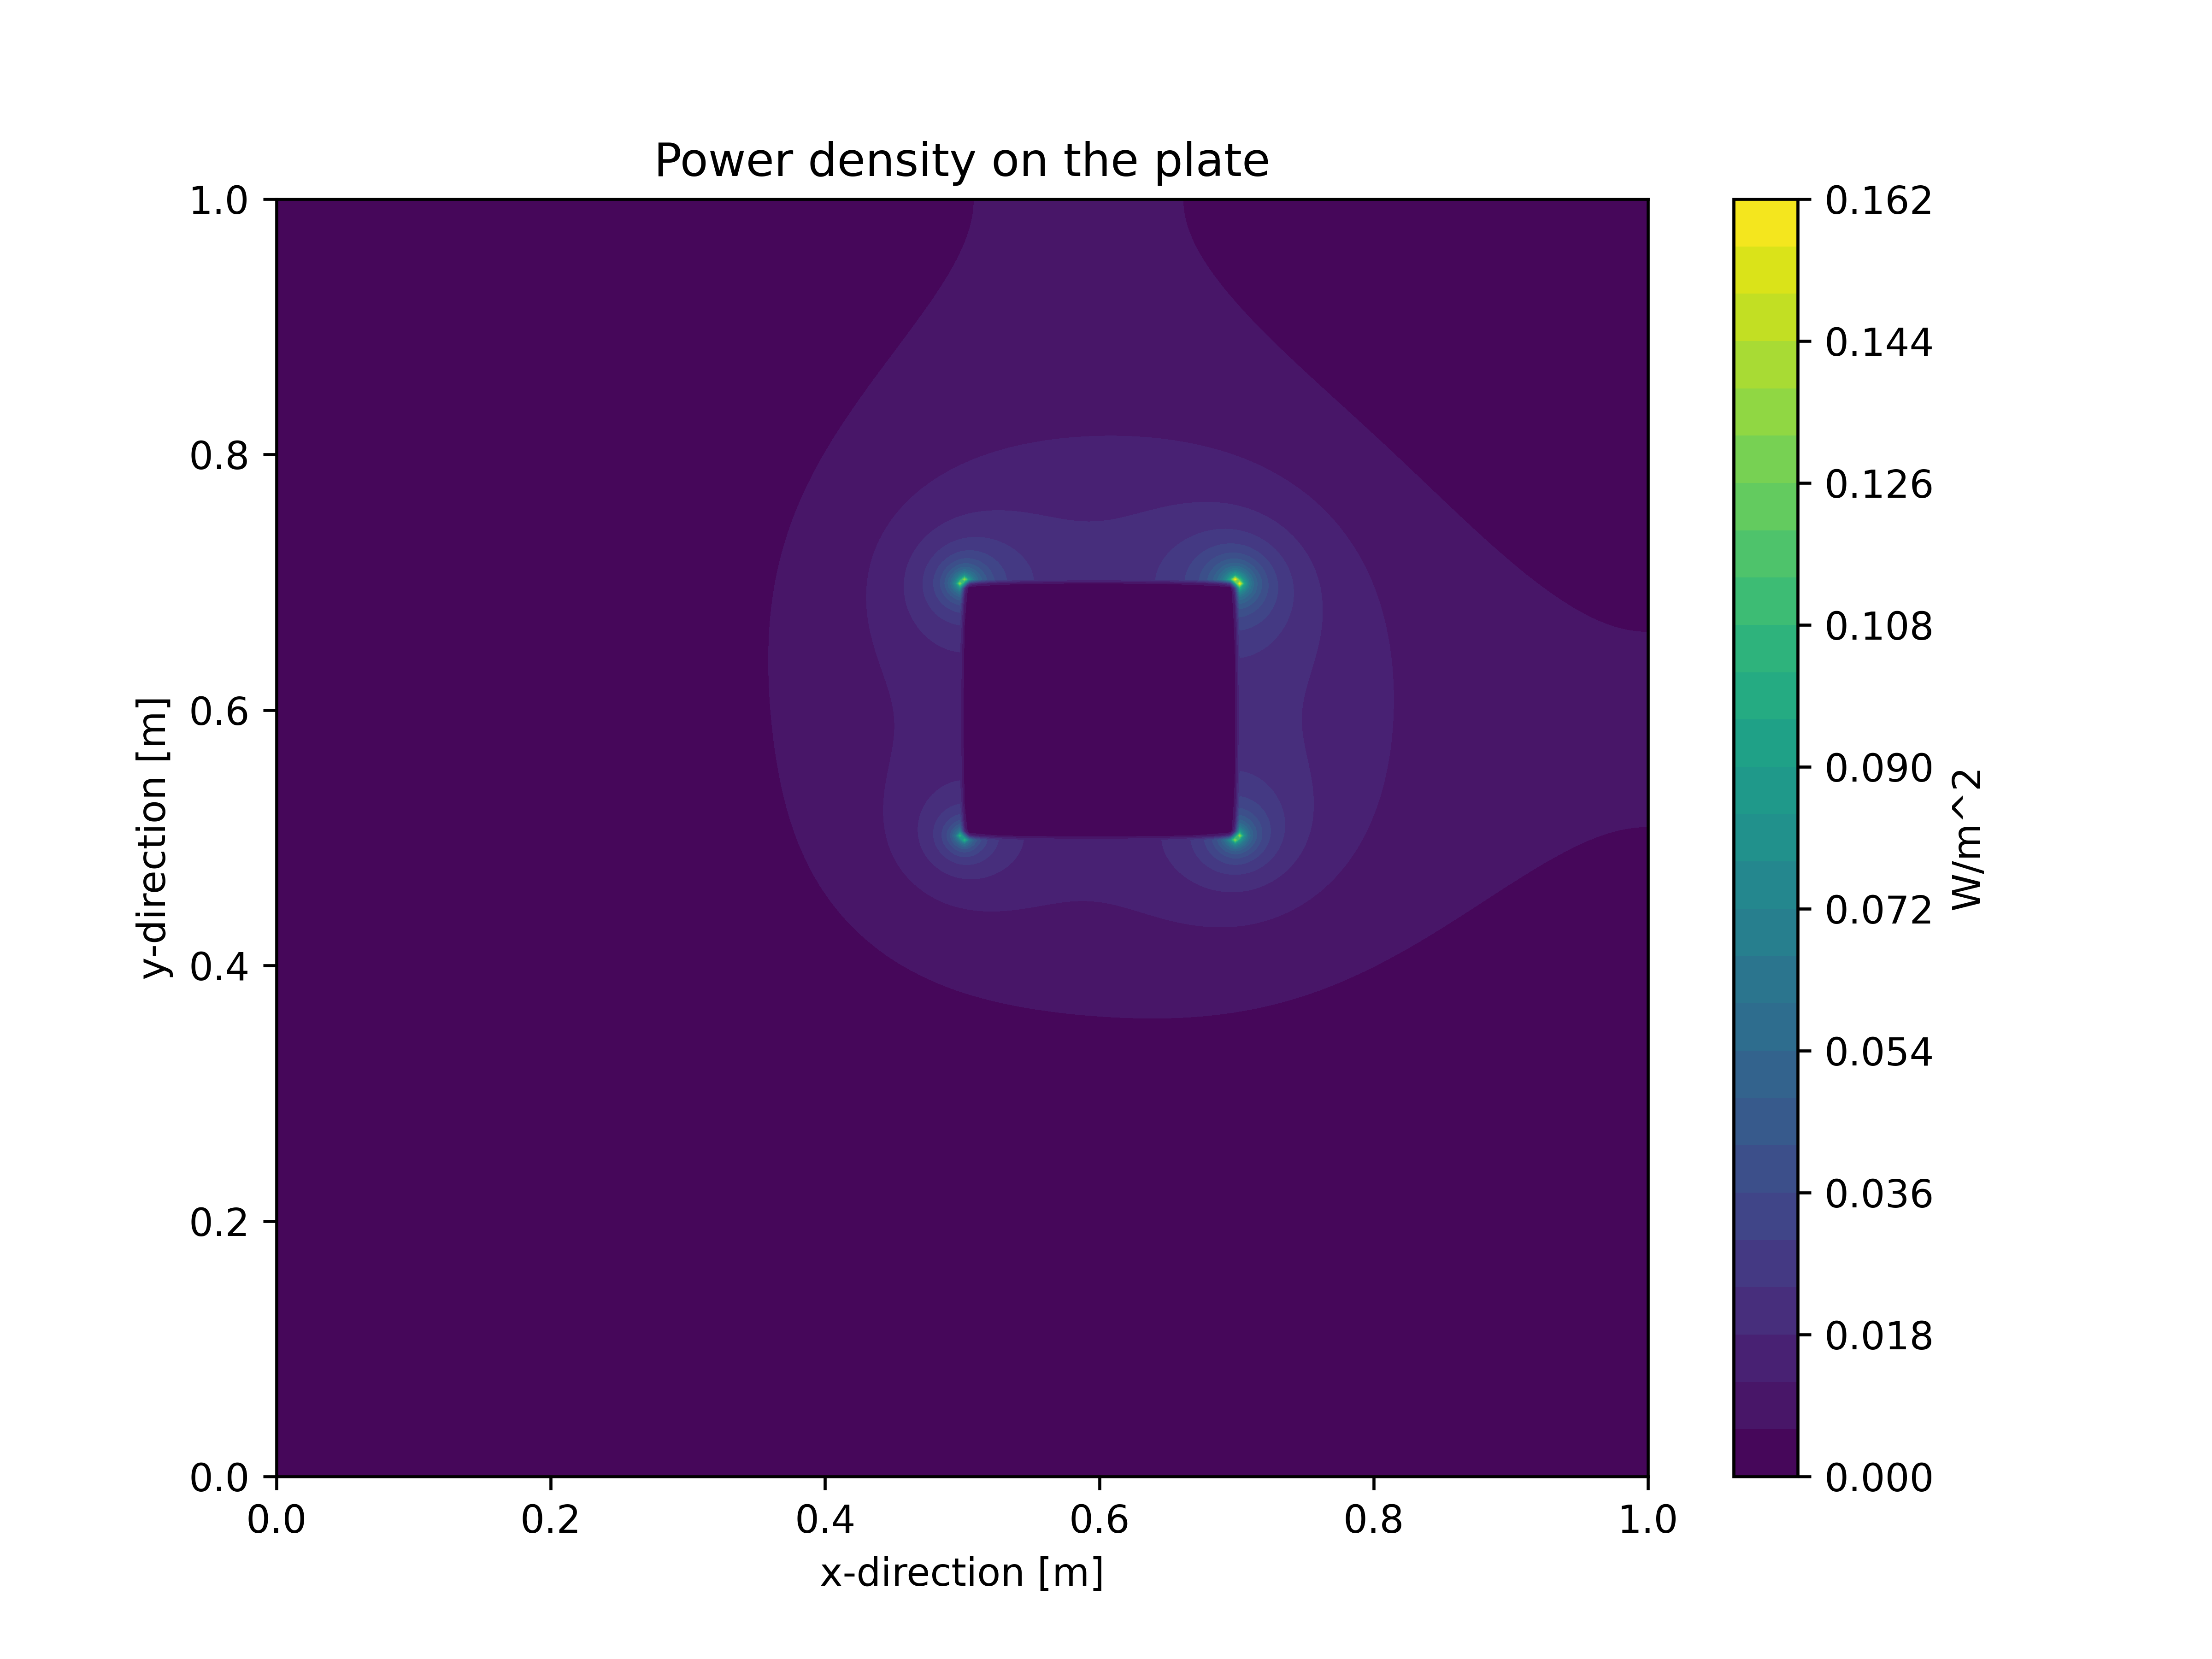
\includegraphics[width=0.99\textwidth]{papers/circuit/power_distribution_circle.png}
	\caption{Leistungsdichte auf rechteckiger Platte mit kreisförmigen Potential im oberen rechten Bereich und 0 Potential am Rand der Platte. (Code für die Generierung des Plots kann in \cite{github:AndreasFMueller} gefunden werden.) }
	\label{fig:power_2d_circle}
\end{figure}
\begin{figure}[h]
	\centering
	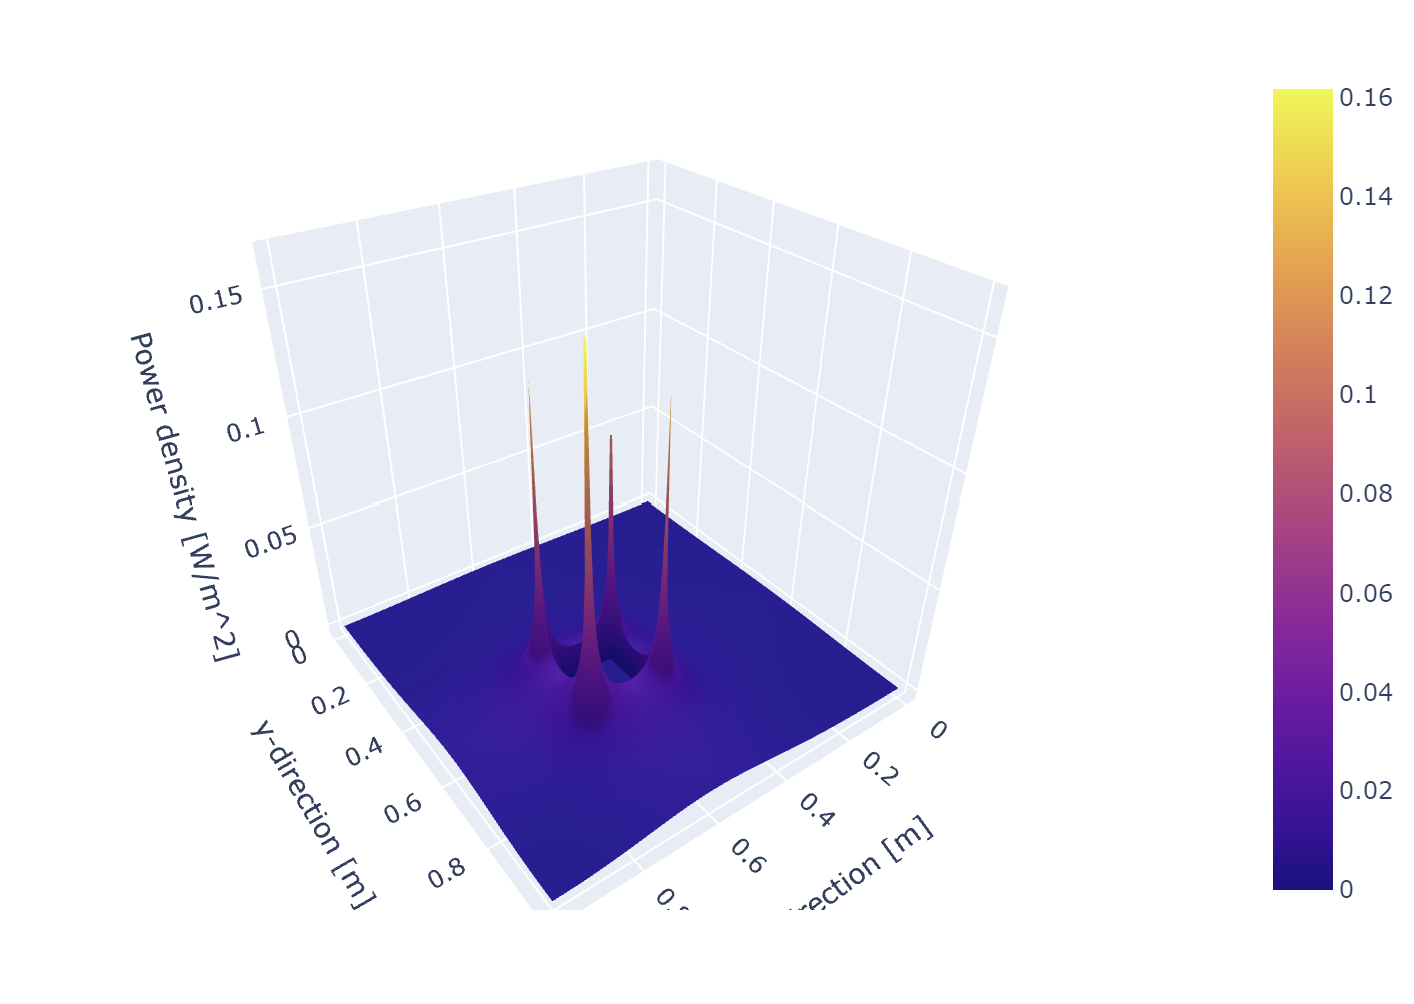
\includegraphics[width=0.99\textwidth]{papers/circuit/3d.png}
	\caption{Leistungsdichte 3d auf rechteckiger Platte mit rechteckigem Potential und 0 Potential am Rand der Platte. (Code für die Generierung des Plots kann in \cite{github:AndreasFMueller} gefunden werden.)}
	\label{fig:power_3d_rectangle}
\end{figure}
\begin{figure}[h]
	\centering
	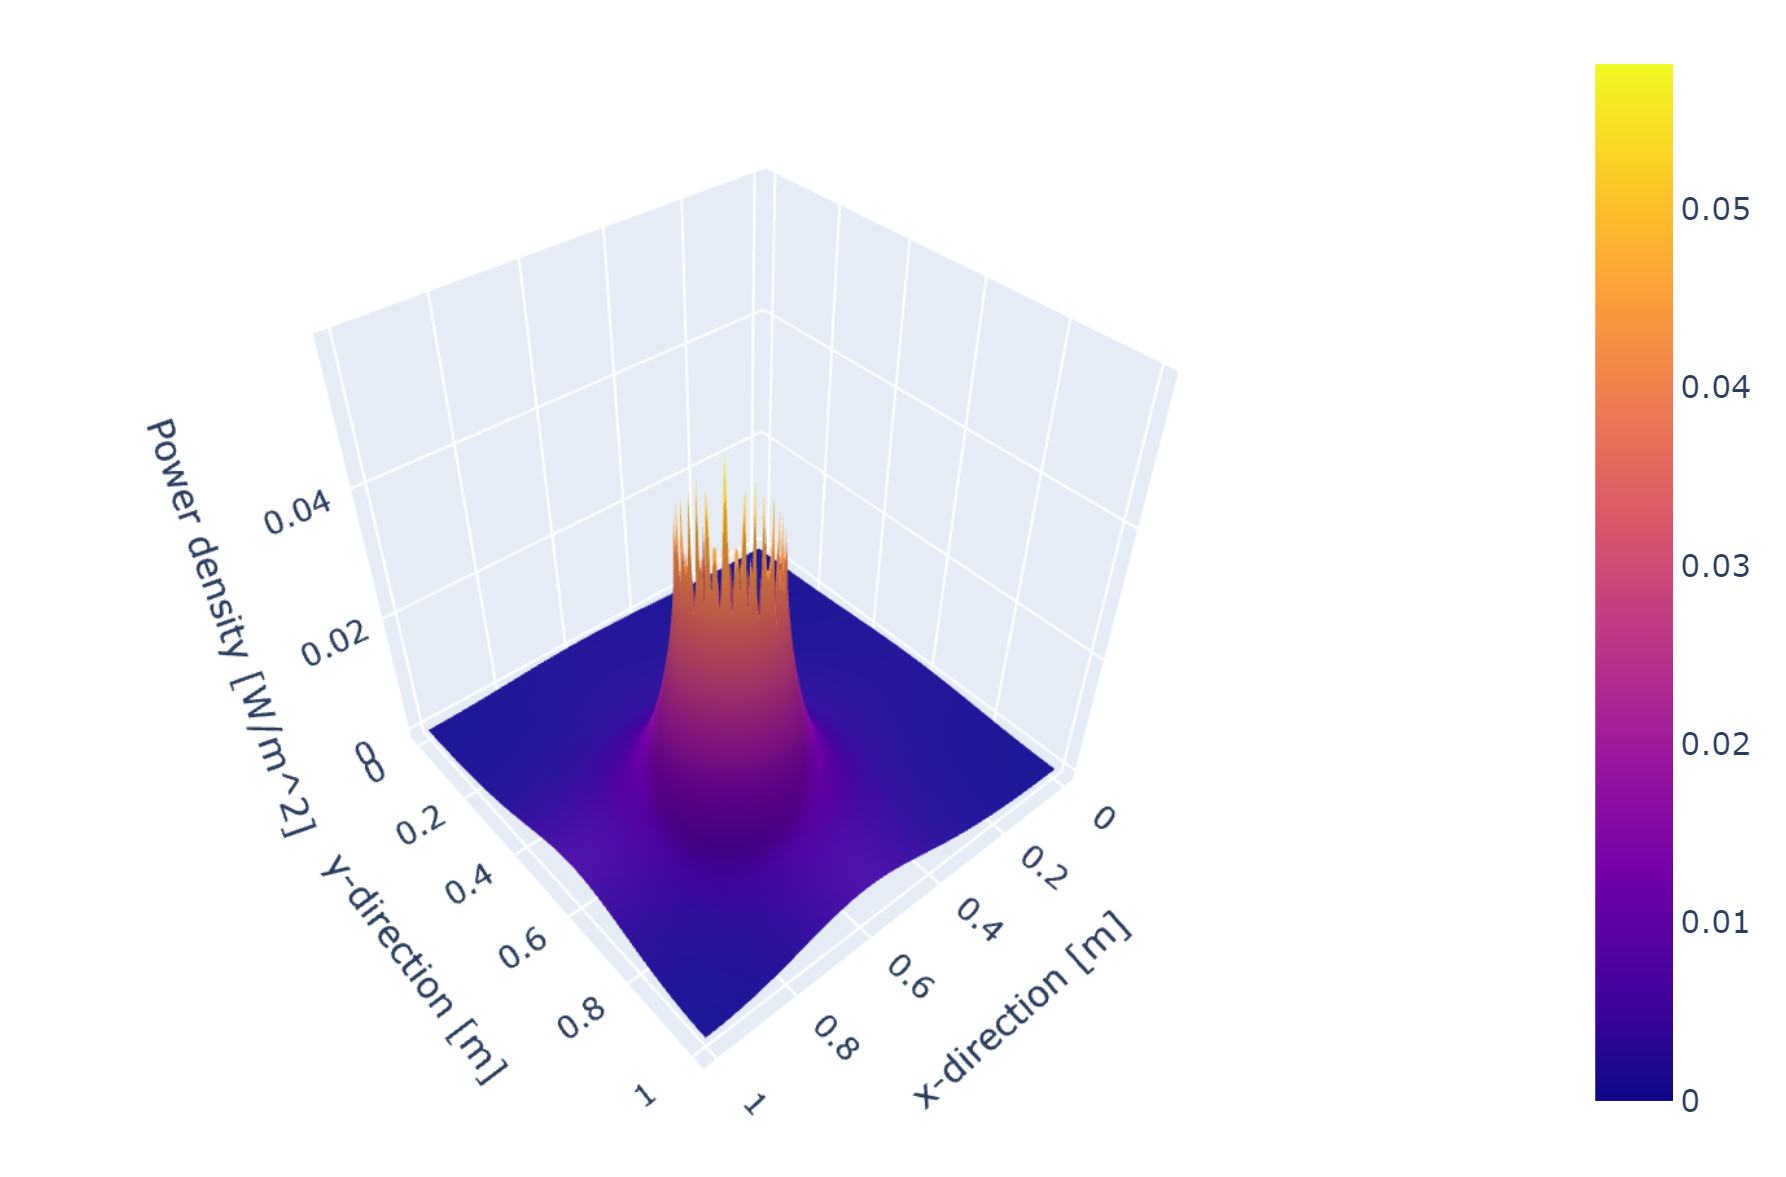
\includegraphics[width=0.99\textwidth]{papers/circuit/3d_circle.png}
	\caption{Leistungsdichte 3d auf rechteckiger Platte mit kreisförmigen Potential und 0 Potential am Rand der Platte. (Code für die Generierung des Plots kann in \cite{github:AndreasFMueller} gefunden werden.)}
	\label{fig:power_3d_circle}
\end{figure}
Abbildung \ref{fig:power_3d_rectangle} zeigt deutlich, dass die Leistungsdichte in den Ecken des zuvor definierten quadratischen Potentials am höchsten ist. Dies ist unter anderem ein Grund, warum auf Leiterplatten normalerweise keine 90°-Winkel für Leiterbahnen gezeichnet werden, sondern meistens 45°-Winkel verwendet werden, um die Leistungsdichte bzw. Stromdichte in den Ecken zu minimieren. 
\subsubsection{Kreisförmiges Potential}
Wird anstatt eines rechteckigen Potentials ein kreisförmiges Potential angelegt, so ist die Leistungsdichte einiges geringer wie es in Abbildung \ref{fig:power_3d_circle} oder Abbildung \ref{fig:power_2d_circle} gesehen werden kann. Wenn man also die Leistungsdichte auf einer Leiterbahn minimieren will verwendet man am besten abgerundete Ecken.
%oder kleine Winkeländerungen, da so der Gradient des Potentials an den Ecken einiges geringer ist.

%Als erstes importieren wir alle nötigen Bibliotheken in Python.
%\begin{lstlisting}[language=Python, caption=Python Librarys]
%"""
%Import the numpy library for numerical computations.
%"""
%import numpy as np
%"""
%Import the matplotlib.pyplot module from the matplotlib library for creating plots and visualizations.
%"""
%import matplotlib.pyplot as plt
%"""
%Import the numba library for just-in-time (JIT) compilation of Python code, which can significantly improve performance.
%"""
%import numba
%"""
%mpl_toolkits.mplot3d is a module from the matplotlib library that provides tools for creating 3D plots and visualizations.
%"""
%from mpl_toolkits.mplot3d import Axes3D
%"""
%matplotlib.cm is a module from the matplotlib library that provides a large set of colormaps for visualizing data in plots.
%"""
%from matplotlib import cm
%\end{lstlisting}
%Anschliessend können wir die Berechnungen anhand von \eqref{circuit:discret_equation3} durchführen, wie es in \eqref{circuit:code1} gezeigt ist \footnote{Der Code wurde mithilfe von Copilot geschrieben}. 
%\begin{lstlisting}[language=Python, caption=Python Librarys, label=circuit:code1]
%def potential_block(x, y):
%	"""
%	Determine the potential value for a given (x, y) coordinate.
%	
%	Parameters:
%	x (float): The x-coordinate.
%	y (float): The y-coordinate.
%	
%	Returns:
%	float: The potential value for the given (x, y) coordinate.
%	"""
%	return np.select([(x>0.5)*(x<0.7)*(y>0.5)*(y<0.7),
%		(x<=0.5)+(x>=0.7)+(y<=0.5)+(y>=0.7)],
%		[1.,
%		0])
%@numba.jit("f8[:,:](f8[:,:], b1[:,:], i8)", nopython=True, nogil=True)
%def compute_potential(potential, fixed_bool, n_iter):
%	"""
%	Compute the potential
%	
%	Parameters:
%	- potential (numpy.ndarray): 2D array representing the potential.
%	- fixed_bool (numpy.ndarray): 2D boolean array indicating fixed points.
%	- n_iter (int): Number of iterations to perform.
%	
%	Returns:
%	- potential (numpy.ndarray): Updated potential after performing the iterations.
%	"""
%	length = len(potential[0])
%	for n in range(n_iter):
%		for i in range(1, length-1):
%			for j in range(1, length-1):
%				if not(fixed_bool[j][i]):
%					potential[j][i] = 1/4 * (potential[j+1][i] + potential[j-1][i] + potential[j][i+1] + potential[j][i-1])
%	return potential
%# define conductivity of the plate (siemens/m)
%sigma = 0.001
%# define size of plate in meters
%width=1
%height=1
%# define number of grid points in one direction
%n=300
%# define grid points
%x = np.linspace(0, width, n)
%y = np.linspace(0, height, n)
%# define potential at boundary points
%upper_y = 0 * x
%lower_y = 0 * x
%upper_x = 0 * y
%lower_x = 0 * y
%# create meshgrid for 2D potential xv are the x coordinates and yv are 
%# the y coordinates at each point, for example xv[0,0] is the x coordinate
%# of the first point and yv[0,0] is the y coordinate of the first point
%xv, yv = np.meshgrid(x, y)
%# create 2d array for potential
%potential = np.zeros((n,n))
%# set potential at boundary points
%potential[0,:]= lower_y
%potential[-1,:]= upper_y
%potential[:,0]= lower_x
%potential[:,-1]= upper_x
%# set potential inside the mesh to a predefined value one
%fixed = potential_block(xv,yv)
%fixed_bool = fixed!=0
%potential[fixed_bool] = fixed[fixed_bool]
%# calculate potential with numberical method and make n_iter iterations
%potential = compute_potential(potential,fixed_bool, n_iter=30000)
%# create a plot of the potential
%fig, ax = plt.subplots(1, 1, figsize=(8,6))
%clr_plot = ax.contourf(xv, yv, potential, 30)
%ax.set_xlabel('x-direction [m]')
%ax.set_ylabel('y-direction [m]')
%fig.colorbar(clr_plot, label='$V$')
%ax.set_title('Potential distribution in the plate')
%plt.show()
%\end{lstlisting}












%Wenn wir den Divergenzsatz/Gauscher Integralsatz (\eqref{circuit:gauscher_integralsatz}) anwenden und \eqref{circuit:current_density_6} verwenden, erhalten wir \eqref{circuit:leistung_gauscher_integralsatz}, da $\sigma$ ein skalar ist und die divergenz vom feld $\phi$ auch kann man den $\nabla$ operator ausklammern und hat die Gleichung dann genau in der Form dass man den satz von Gaus anwwenden kann.
%\begin{equation}
%	\oint_S \vec{F}_i \cdot \mathrm{d} \vec{S}=\int_V \nabla \cdot \vec{F}_i \mathrm{~d} V
%	\label{circuit:gauscher_integralsatz}
%\end{equation}
%
%
%
%
%
%
%
%\begin{equation}
%P=\int_V \nabla \cdot(\sigma \phi \nabla \phi) d V=\oint_S(\sigma \phi \nabla \phi) \cdot d \vec{S}
%\label{circuit:leistung_gauscher_integralsatz}
%\end{equation}
%
%Wenn die Leitfähigkeit im gesamten Volumen $V$ konstant ist, wird die Variation der Wärmeerzeugungsrate $P$ in $V$ gegeben durch \eqref{circuit:leistung_gauscher_integralsatz2}. Auf diese form der Gleichung kommt man wenn man das Kommutativgesetz und anschliessend die produkteregel  auf \eqref{circuit:leistung_gauscher_integralsatz} anwendet, wie es in \eqref{eq:produkteregel} gezeigt ist. Dabei ist zu beachten dass partielle Ableitungen für stetig differenzierbare funktionen vertauschbar sind ($\phi \nabla(\delta \phi) = \phi \delta(\nabla \phi)$).
%\begin{equation}
%\delta P=\sigma \oint_S(\delta \phi \nabla \phi) \cdot d \vec{S}+\sigma \oint_S(\phi \nabla(\delta \phi)) \cdot d \vec{S}
%\label{circuit:leistung_gauscher_integralsatz2}
%\end{equation}
%
%$$
%\delta[y(x)]=\bar{y}(x)-y(x)=\varepsilon\eta(x)
%$$
%
%
%\begin{equation}
%	\begin{aligned}
%		\delta P &=\sigma \cdot \delta \oint_S( \phi \nabla \phi) \cdot d \vec{S} = \sigma \cdot \oint_S \delta(\underbrace{\phi}_{u} \underbrace{\nabla \phi}_{v}) \cdot d \vec{S}\\
%		&= \sigma \cdot \oint_S \left(\underbrace{(\delta \phi)}_{u'} \cdot  \underbrace{(\nabla \phi)}_{v} + \underbrace{\phi}_{u} \cdot  \underbrace{\delta(\nabla \phi)}_{v'}\right)\cdot d \vec{S}
%	\end{aligned}
%	\label{eq:produkteregel}
%\end{equation}
%
%Nun haben wir die Gleichung gefunden und wir können die Euler-Ostrogradski-Differentialgleichung aus \cite{circuit:paper1} welche auch in \eqref{circuit:euler_lagransky} zu finden anwenden
%
%\begin{equation}
%	\textcolor{orange}{\frac{\partial F}{\partial z}(x, y, \phi, \frac{\partial \phi}{\partial x}, \frac{\partial \phi}{\partial y})}-\textcolor{brown}{\frac{\partial}{\partial x} \frac{\partial F}{\partial z_x}(x, y, \phi, \frac{\partial \phi}{\partial x}, \frac{\partial \phi}{\partial y})}-\textcolor{violet}{\frac{\partial}{\partial y} \frac{\partial F}{\partial z_y}(x, y, \phi, \frac{\partial \phi}{\partial x}, \frac{\partial \phi}{\partial y})}=0
%	\label{circuit:euler_lagransky}
%\end{equation}
%Machen wir das für den ersten teil der Gleichung und nehemen an das $\phi$ zwei dimensional ist und daher folgendes gilt $\phi=\phi(x,y)$
%\begin{equation}
%	\delta P=\sigma \oint_S(\delta \phi \nabla \phi) \cdot d \vec{S} \textcolor{gray}{+\sigma \oint_S(\phi \nabla(\delta \phi)) \cdot d \vec{S}}
%	\label{circuit:calc1}
%\end{equation}
%Wenn  wir die Formel nun anwenden kommen wir auf folgendes, da $\phi$ in der gleichung nur als ableitung vorkommt.
%\begin{equation}
%	\textcolor{orange}{\frac{\partial P}{\partial z}(x, y, \phi, \frac{\partial \phi}{\partial x}, \frac{\partial \phi}{\partial y})=0}
%\end{equation}
%\begin{equation}
%	\nabla=\frac{\partial}{\partial z} i+\frac{\partial}{\partial y} j+\frac{\partial}{\partial z} k
%	\label{circuit:nabla_operator}
%\end{equation}
%\begin{equation}
%	\textcolor{brown}{\frac{\partial}{\partial x}\frac{\partial P}{\partial \frac{\partial \phi}{\partial x}}(x, y, \phi, \frac{\partial \phi}{\partial x}, \frac{\partial \phi}{\partial y})
%	=\frac{\partial}{\partial x}\frac{\partial}{\partial \frac{\partial \phi}{\partial x}}\left(\delta \phi \left(\frac{\partial \phi}{\partial x} i+\frac{\partial \phi}{\partial y} j\right)\right)
%	=\frac{\partial}{\partial x}\left(\delta \phi \left(1+0\right)\right)}
%\end{equation}
%
%\begin{equation}
%	\textcolor{violet}{\frac{\partial}{\partial y}\frac{\partial P}{\partial \frac{\partial \phi}{\partial y}}(x, y, \phi, \frac{\partial \phi}{\partial x}, \frac{\partial \phi}{\partial y})
%	=\frac{\partial}{\partial y}\frac{\partial}{\partial \frac{\partial \phi}{\partial y}}\left(\delta \phi \left(\frac{\partial \phi}{\partial x} i+\frac{\partial \phi}{\partial y} j\right)\right)
%	=\frac{\partial}{\partial y}\left(\delta \phi \left(0+1\right)\right)}
%\end{equation}
%
%Setzen wir wieder alls zusammen bekommen wir folgendes:
%\begin{equation}
%	\textcolor{orange}{0}-\textcolor{brown}{\frac{\partial}{\partial x}\left(\delta \phi \left(1+0\right)\right)} - \textcolor{violet}{\frac{\partial}{\partial y}\left(\delta \phi \left(0+1\right)\right)}=0
%\end{equation}
%
%\begin{equation}
%	\Delta \phi(x,y)=\frac{\delta^2\phi}{\delta x^2}+\frac{\delta^2\phi}{\delta y^2}=0
%\end{equation}
%\begin{equation}
%	\Delta h(x)=0
%\end{equation}
%
%
%
%Aus \eqref{circuit:leistung_gauscher_integralsatz2} geht hervor, dass wenn Variationen im Fluss, $\delta \phi$, an der Grenze von $V$ verschwinden, dann ist $P$ stationär, d.h. $\delta P=0$. Daher werden elektrische Ströme in der Region verteilt, mit einer angelegten Spannung an ihrer Grenze,
%
%
%\begin{figure}
%	\centering
%	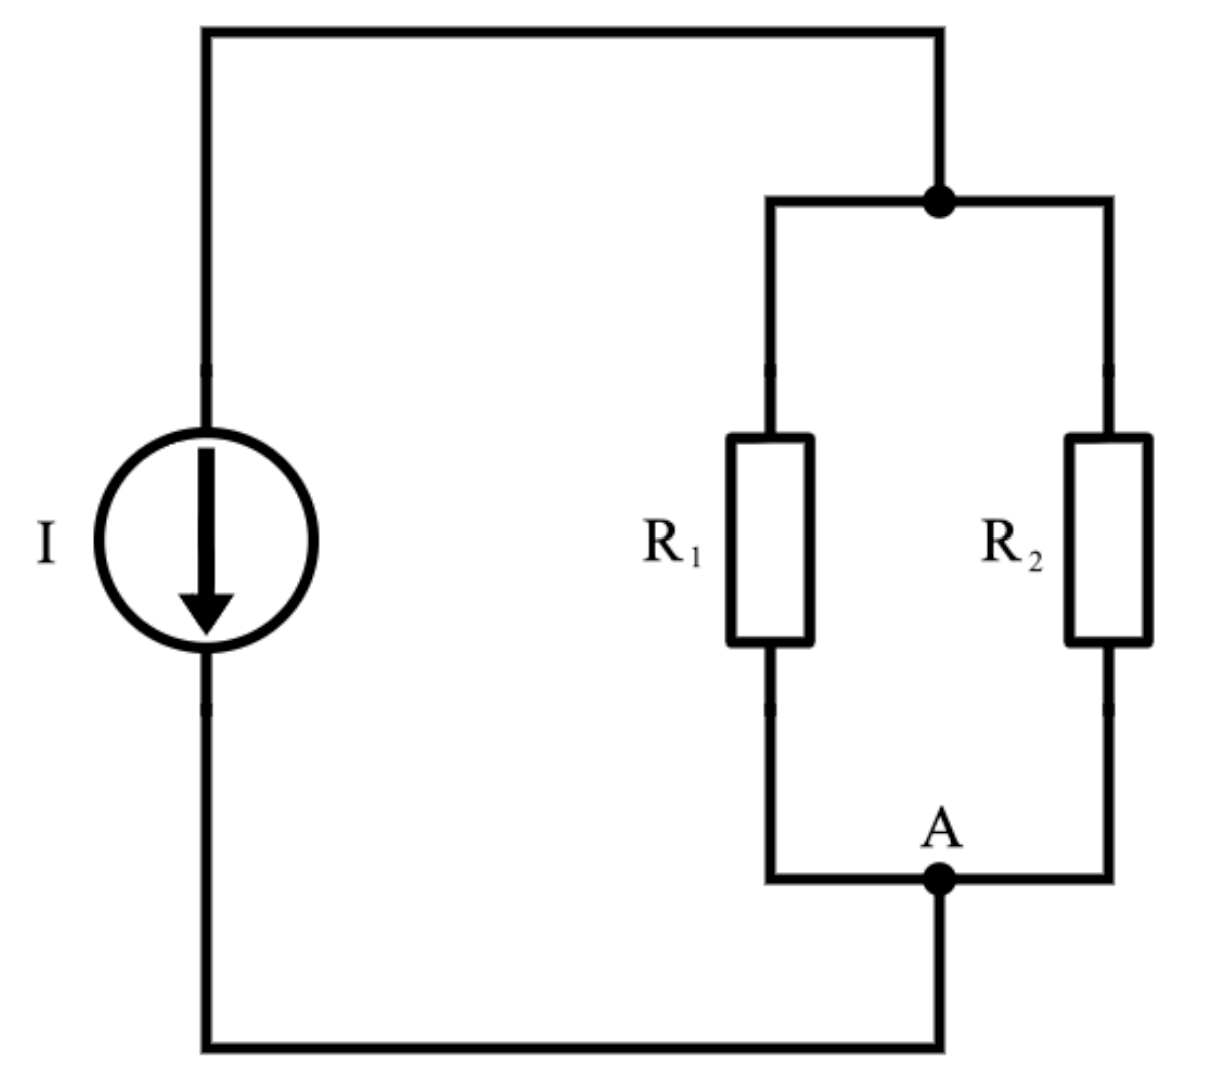
\includegraphics[width=0.6\textwidth]{papers/circuit/images/image_01.png}
%	\caption{Parrallelschaltung von zwei Wiederständen \cite{circuit:bibtex}
%	\label{papers:circuit:images:parallelschaltung_strom}}
%\end{figure}




%https://www.youtube.com/watch?v=VCHFCXgYdvY
